\newpage

\section{Finally, let us compare both estimation methods (MLE and MOM). To this end, set the number of simulations equal to $Nsim = 1500$.}


% -------------------------------------------------------------------------------------------------

\subsection*{(a) Use the previous implementation for the MOM and use the function \texttt{ebeta} contained in the package \texttt{EnvStats} for the MLE estimator for the beta distribution to create histograms illustrating the distribution of each of the shape parameters.}

We conducted \(N_{sim} = 1500\) independent simulations, each generating \(n = 15,\!000\) samples from a \(\text{Be}(9, 3)\) distribution. For each simulated dataset, we estimated the shape parameters \(\alpha\) and \(\beta\) using two methods:

\begin{itemize}
    \item Maximum likelihood estimation (MLE): Using the \texttt{beta.fit} function from the \texttt{scipy.stats} library, which estimates parameters by maximizing the likelihood function.
    \item Method of moments (MOM): Based on equating the theoretical moments of the Beta distribution to the sample moments.
\end{itemize}

\vspace{0.5em}
The histograms (Figure \ref{fig:q11a-beta_parameter_estimations}) illustrate the empirical distribution of the estimated parameters across the 1500 simulations.

\begin{figure}[H]
    \centering
    \begin{subfigure}[b]{0.48\textwidth}
        \centering
        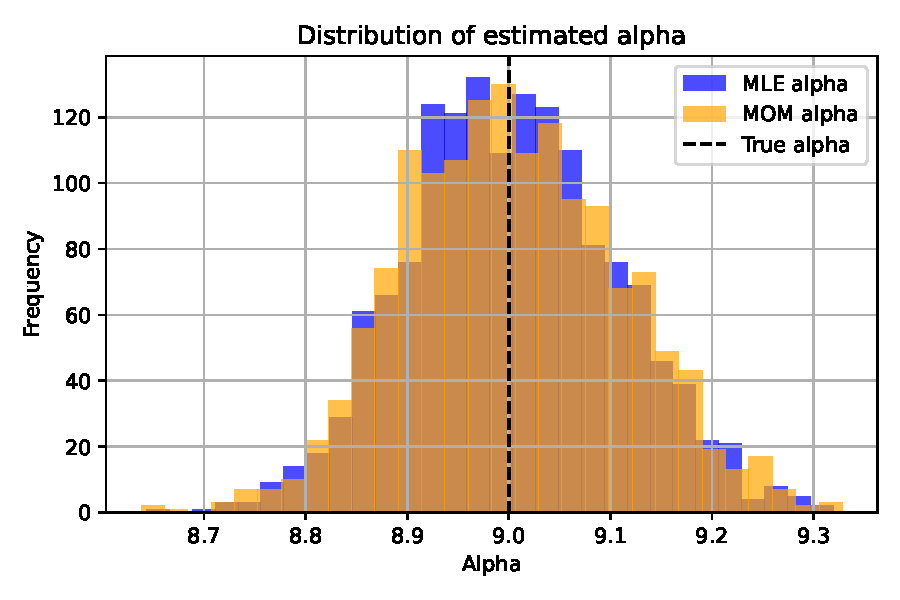
\includegraphics[width=\textwidth]{resources/figures/q11a-estimated_alpha_histogram.pdf}
        \caption{Estimated \(\alpha\) values}
        \label{fig:alpha_hist}
    \end{subfigure}
    \hfill
    \begin{subfigure}[b]{0.48\textwidth}
        \centering
        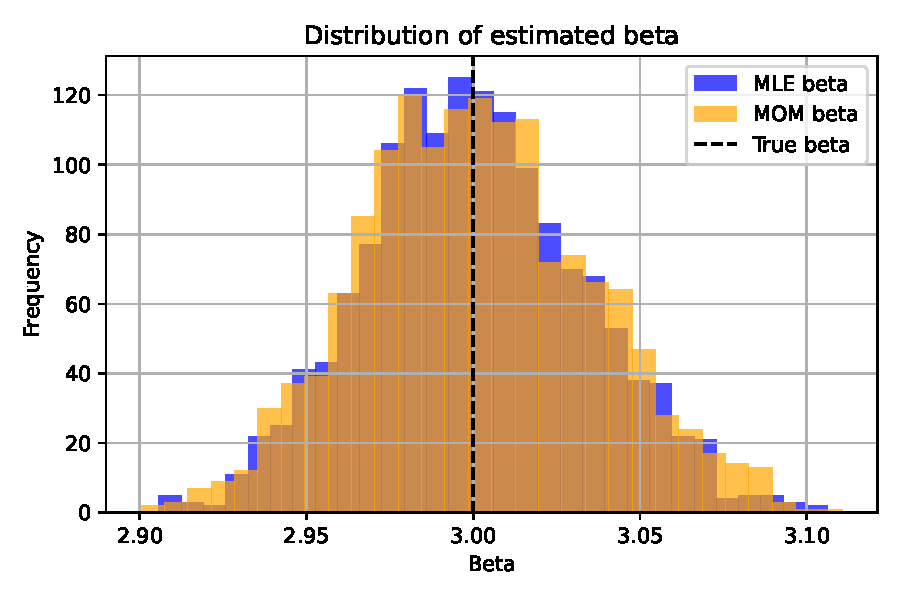
\includegraphics[width=\textwidth]{resources/figures/q11a-estimated_beta_histogram.pdf}
        \caption{Estimated \(\beta\) values}
        \label{fig:beta_hist}
    \end{subfigure}
    \caption{Histograms of estimated Beta distribution parameters across 1500 simulations.} % Blue bars: MLE estimates; orange bars: MOM estimates; dashed lines indicate true parameter values (\(\alpha=9\), \(\beta=3\)).}
    \label{fig:q11a-beta_parameter_estimations}
\end{figure}


% \vspace{0.5em}
% \textbf{Interpretation:} 

% Regarding Figure \ref{fig:q11a-beta_parameter_estimations}:
\begin{itemize}
    \item Both the MLE and MOM estimators for \(\alpha\) and \(\beta\) are approximately unbiased, with distributions centered near the true parameter values.
    \item The spread of the histograms indicates the variability of the estimators. Visual inspection suggests that the MLE estimators have slightly less variability than the MOM estimators.
    \item The overlap in histograms indicates strong agreement between the two estimation methods for large samples.
\end{itemize}

% These results provide a visual understanding of the sampling distributions of the estimators and lay the foundation for quantitative evaluation of efficiency in the subsequent part (b).



% In Python, we can use the \texttt{fit} function to estimate the parameter using the MLE technique. I simulated 100 parameters for both $\alpha$ and $\beta$. The histograms are shown below:

% \begin{figure}[h]
%     \centering
%     \begin{minipage}{0.45\textwidth}
%         \centering
%         % \includegraphics[width=\textwidth]{histogram_alpha.pdf} % Replace with actual filename
%         \caption*{(a) alpha}
%     \end{minipage}
%     \hfill
%     \begin{minipage}{0.45\textwidth}
%         \centering
%         % \includegraphics[width=\textwidth]{histogram_beta.pdf} % Replace with actual filename
%         \caption*{(b) beta}
%     \end{minipage}
%     \caption{Histogram of the estimated parameter using MOM and MLE}
%     \label{fig:hist-mom-mle}
% \end{figure}


% -------------------------------------------------------------------------------------------------
\newpage
\subsection*{(b) Evaluate the efficiency of each method in terms of bias and variance. Compare the results.}

Using the simulation results from $1,\!500$ independent datasets of size \(n = 15,\!000\) drawn from a \(\text{Be}(9, 3)\) distribution, we evaluated the bias and variance of the shape parameter estimators for both Maximum Likelihood Estimation (MLE) and Method of Moments (MOM).

The results are summarized in Table \ref{tab:q11b}:

\begin{table}[H]
\centering
\footnotesize
\noskipcaption{Estimated bias and variance of the Beta distribution shape parameters over 1500 simulations.}
\label{tab:q11b}
\begin{tabular}{lcc}
\hline
\textbf{Parameter} & \textbf{Bias} & \textbf{Variance} \\
\hline
\(\alpha\) (MLE) & \(0.002573\) & \(0.010503\) \\
\(\alpha\) (MOM) & \(0.003619\) & \(0.011518\) \\
\hline
\(\beta\) (MLE) & \(0.000461\) & \(0.001087\) \\
\(\beta\) (MOM) & \(0.000858\) & \(0.001211\) \\
\hline
\end{tabular}
\end{table}

\begin{itemize}
    \item Both MLE and MOM estimators exhibit very small biases, indicating nearly unbiased estimation of the parameters.
    \item The MLE estimators have slightly lower variance for both \(\alpha\) and \(\beta\), suggesting higher efficiency compared to the MOM estimators.
    \item Overall, both methods provide accurate and reliable parameter estimates for large samples, with MLE being marginally preferable in terms of variability.
\end{itemize}



% ---

% The histogram of the variance and bias are displayed below:

% \begin{figure}[h]
%     \centering
%     \begin{minipage}{0.45\textwidth}
%         \centering
%         % \includegraphics[width=\textwidth]{bias_alpha.pdf} % Replace with actual filename
%         \caption*{(a) bias alpha}
%     \end{minipage}
%     \hfill
%     \begin{minipage}{0.45\textwidth}
%         \centering
%         % \includegraphics[width=\textwidth]{bias_beta.pdf} % Replace with actual filename
%         \caption*{(b) bias beta}
%     \end{minipage}

%     \vspace{1em}

%     \begin{minipage}{0.45\textwidth}
%         \centering
%         % \includegraphics[width=\textwidth]{variance_alpha.pdf} % Replace with actual filename
%         \caption*{(c) variance alpha}
%     \end{minipage}
%     \hfill
%     \begin{minipage}{0.45\textwidth}
%         \centering
%         % \includegraphics[width=\textwidth]{variance_beta.pdf} % Replace with actual filename
%         \caption*{(d) variance beta}
%     \end{minipage}

%     \caption{Histogram of the variance and bias of the different parameters using MOM and MLE}
%     \label{fig:variance-bias}
% \end{figure}

% \vspace{1em}

% \begin{table}[h]
%     \centering
%     \begin{tabular}{|c|c|c|}
%         \hline
%         \textbf{Param} & \textbf{MOM} & \textbf{MLE} \\
%         \hline
%         Alpha & -0.00017 & -0.00020 \\
%         Beta  & -0.0025  & -0.00242 \\
%         \hline
%     \end{tabular}
%     \caption{Bias}
%     \label{tab:bias}
% \end{table}

% \vspace{1em}

% \begin{table}[h]
%     \centering
%     \begin{tabular}{|c|c|c|}
%         \hline
%         \textbf{Param} & \textbf{MOM} & \textbf{MLE} \\
%         \hline
%         Alpha & 0.00579 & 0.00558 \\
%         Beta  & 0.03489 & 0.0343 \\
%         \hline
%     \end{tabular}
%     \caption{Variance}
%     \label{tab:variance}
% \end{table}

% \vspace{1em}

% Comparing the histogram and the tables for the bias and variance for both methods (MLE and MOM), I have the same results, meaning that both methods perform equally well on the task of estimating the shape parameters of a beta distribution. 

% This is surprising, because we know that MLE has a biased variance estimator while MOM has an unbiased one. Knowing those facts, we should have different results for the variance at least.


% -------------------------------------------------------------------------------------------------
% \newpage
\subsection*{(c) Illustrate the asymptotic normality of the obtained MLE estimators.}

The asymptotic normality property is fundamental in statistics and describes how, as the sample size \(n\) grows large, the distribution of the maximum likelihood estimator (MLE) \(\hat{\theta}\) approaches a normal distribution centered around the true parameter \(\theta_{\text{true}}\).

Mathematically, this is expressed as:
\[
\sqrt{n}(\hat{\theta} - \theta_{\text{true}}) \xrightarrow{d} \mathcal{N}\left(0, \sigma^2_{\hat{\theta}, \text{true}}\right),
\]
where \(\xrightarrow{d}\) denotes convergence in distribution, and \(\sigma^2_{\hat{\theta}, \text{true}}\) is the asymptotic variance of the estimator.

In this context:
\begin{itemize}
    \item \(\sqrt{n}\) represents the rate at which the distribution converges.
    \item \(\hat{\theta}\) is the estimator obtained from the data.
    \item \(\theta_{\text{true}}\) is the true (unknown) parameter value.
\end{itemize}

\vspace{0.5em}
Using \(N_{sim} = 1500\) simulations of sample size \(n = 15,000\) from a \(\text{Be}(9, 3)\) distribution, we computed MLE estimates for the shape parameters \(\alpha\) and \(\beta\).

Figure~\ref{fig:mle_histograms} and Figure~\ref{fig:mle_qqplots} illustrate that the distribution of the scaled estimation errors \(\sqrt{n}(\hat{\theta} - \theta_{\text{true}})\) approximates a normal distribution centered around zero, which confirms the asymptotic normality of the MLE estimators.

\begin{figure}[H]
    \centering
    \begin{subfigure}[b]{0.48\textwidth}
        \centering
        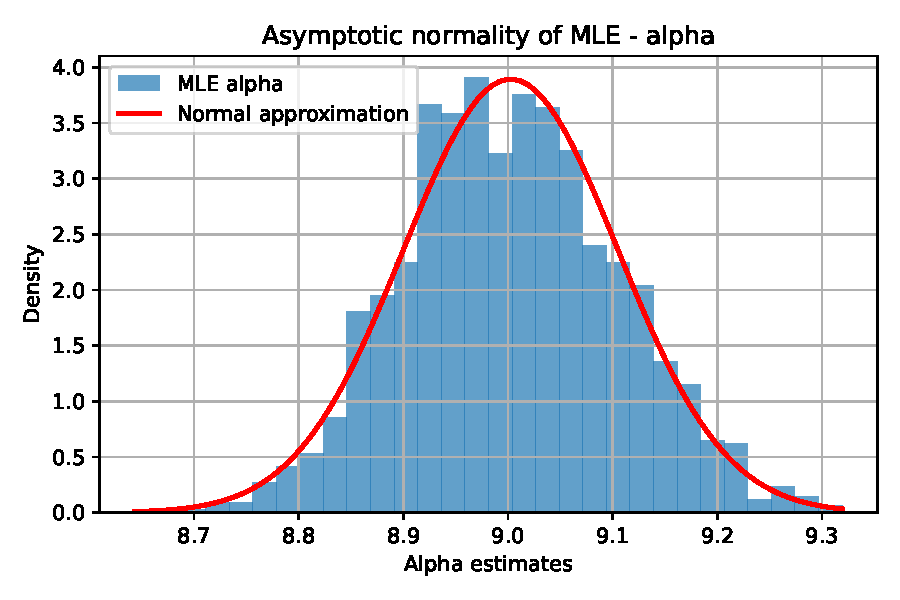
\includegraphics[width=\textwidth]{resources/figures/q11c-alpha_mle_histogram.pdf}
        \caption{Histogram of MLE \(\alpha\) estimates with normal overlay}
        \label{fig:mle_alpha_hist}
    \end{subfigure}
    \hfill
    \begin{subfigure}[b]{0.48\textwidth}
        \centering
        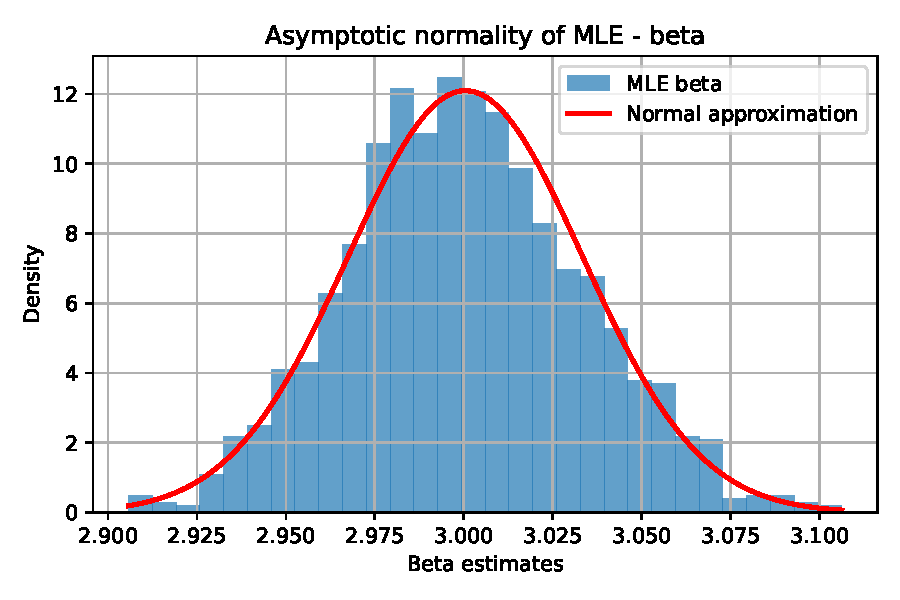
\includegraphics[width=\textwidth]{resources/figures/q11c-beta_mle_histogram.pdf}
        \caption{Histogram of MLE \(\beta\) estimates with normal overlay}
        \label{fig:mle_beta_hist}
    \end{subfigure}
    \caption{Histograms illustrating the approximate normality of MLE estimators for Beta parameters \(\alpha\) and \(\beta\).}
    \label{fig:mle_histograms}
\end{figure}

The empirical distribution of the MLE estimates for \(\alpha\) and \(\beta\) closely resemble normal distributions (red curves) with means and variances matching the sample estimates.

\begin{figure}[H]
    \centering
    \begin{subfigure}[b]{0.48\textwidth}
        \centering
        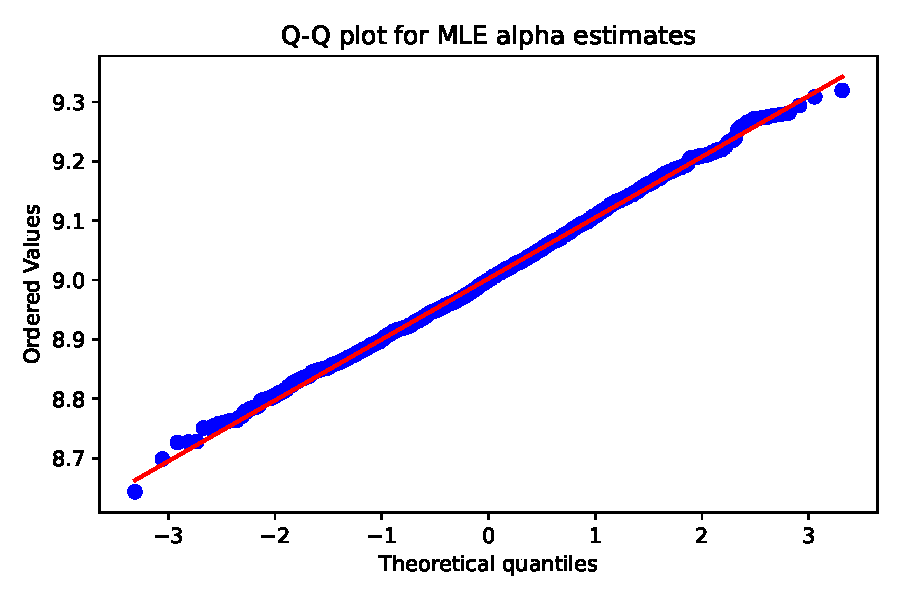
\includegraphics[width=\textwidth]{resources/figures/q11c-alpha_mle_qqplot.pdf}
        \caption{Q-Q plot for MLE \(\alpha\) estimates}
        \label{fig:mle_alpha_qq}
    \end{subfigure}
    \hfill
    \begin{subfigure}[b]{0.48\textwidth}
        \centering
        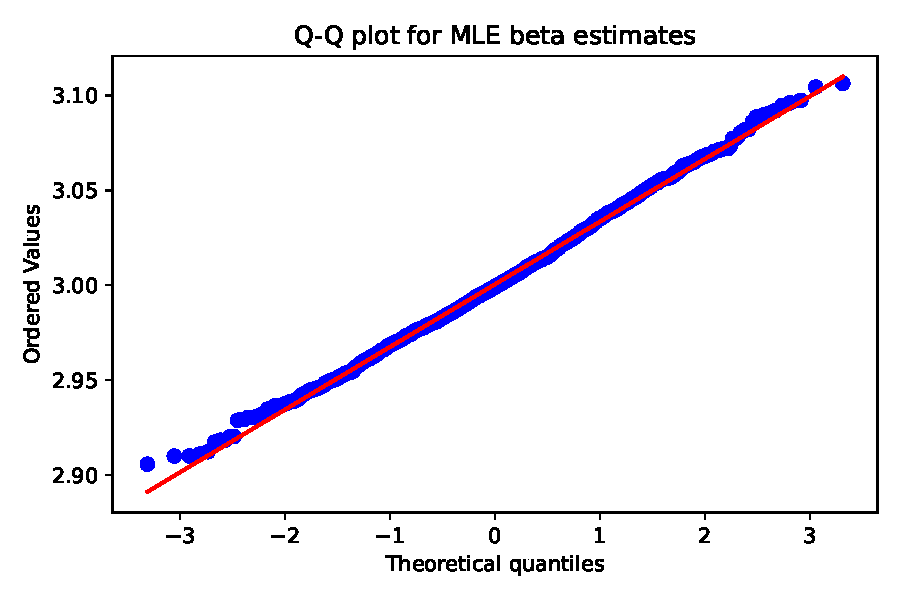
\includegraphics[width=\textwidth]{resources/figures/q11c-beta_mle_qqplot.pdf}
        \caption{Q-Q plot for MLE \(\beta\) estimates}
        \label{fig:mle_beta_qq}
    \end{subfigure}
    \caption{Q-Q plots comparing empirical quantiles of MLE estimators to theoretical normal quantiles, showing good agreement.}
    \label{fig:mle_qqplots}
\end{figure}

The quantile-quantile plots compare the quantiles of the MLE estimates to those of a theoretical normal distribution. The points fall approximately along the diagonal line, indicating that the empirical distributions are well-approximated by normal distributions.

These visualizations clearly demonstrate that, as the number of simulations increases, the distribution of estimation errors tends toward a normal distribution centered at zero, consistent with the asymptotic normality property of MLE estimators.



% An illustration of this phenomenon is displayed in the following plots:

% \begin{figure}[h]
%     \centering
%     \begin{minipage}{0.45\textwidth}
%         \centering
%         % \includegraphics[width=\textwidth]{asymptotic_100.pdf} % Replace with actual filename
%         \caption*{(a) Nsim = 100}
%     \end{minipage}
%     \hfill
%     \begin{minipage}{0.45\textwidth}
%         \centering
%         % \includegraphics[width=\textwidth]{asymptotic_1000.pdf} % Replace with actual filename
%         \caption*{(b) Nsim = 1000}
%     \end{minipage}
    
%     \vspace{1em}
    
%     \begin{minipage}{0.45\textwidth}
%         \centering
%         % \includegraphics[width=\textwidth]{asymptotic_10000_alpha.pdf} % Replace with actual filename
%         \caption*{(c) Nsim = 10000}
%     \end{minipage}
%     \hfill
%     \begin{minipage}{0.45\textwidth}
%         \centering
%         % \includegraphics[width=\textwidth]{asymptotic_10000_beta.pdf} % Replace with actual filename
%         \caption*{(d) Nsim = 10000}
%     \end{minipage}
    
%     \caption{Phenomenon of the asymptotic normality illustration, for increasing number of simulations}
%     \label{fig:asymptotic-normality}
% \end{figure}

% The \textit{asymptotic normality} is a property of an estimator when the sample size gets infinitely large. It is very similar to the central limit theorem. This property consists in converging weakly to a normal distribution. Mathematically, an estimator has asymptotic normality if the following equation holds:

% \[
% \sqrt{n}(\hat{\theta} - \theta_{\text{true}}) \xrightarrow{d} \mathcal{N}(0, \sigma^2_{\hat{\theta}, \text{true}})
% \]

% $\sqrt{n}$ corresponds to the speed of convergence, while $\theta_{\text{true}}$ and $\hat{\theta}$ correspond respectively to the true parameter and the MLE estimator.

% \vspace{0.5em}

% We clearly see, as the number of simulations becomes larger, that the distribution of the difference between the true value of the parameters and the estimations tends to a normal distribution centered at 0.





